\documentclass{article}
\usepackage{graphicx}
\usepackage[margin=2.5cm]{geometry}
\usepackage{listings}
\lstset{language=Python}
\usepackage{hyperref}
\usepackage{minted}
\usepackage{amsmath}
\usepackage{tikz, pgfplots}
\usetikzlibrary{positioning}
\usepackage{parskip}
\usepackage{adjustbox}
\usepackage{amssymb}

\begin{document}

\title{
    {Linear Algebra Project: Image Compression}\\
    {\large International Institute of Information Technology, Hyderabad}\\
    \author{Vinit Mehta, Swarang Joshi, Nijesh Raghava}
    \vspace{1cm}
    
\includegraphics[width=3cm]{IIITH.png}
}
\date{}

\maketitle

\section{Introduction}
Image compression is a fundamental technique in the field of computer vision and image processing. It plays a crucial role in reducing the storage requirements and transmission bandwidth for images without significant loss in visual quality. Over the years, numerous image compression techniques have been developed, aiming to achieve higher compression ratios while maintaining good perceptual quality. In recent years advanced algorithms and approaches to push the boundaries of image compression performance have emerged. This thesis focuses on exploring the use of Principal Component Analysis (PCA), Vector Quantization, Discrete Cosine Transform(DCT) and Wavelet Transform.

\subsection{SVD}
Image compression using Singular Value Decomposition (SVD) has been an active area of research, and several recent updates have focused on enhancing compression efficiency and image quality. Here are some notable advancements in the field of image compression using SVD:

\begin{itemize}
  \item {\textbf{Adaptive SVD-based Compression:} Traditional SVD-based compression methods use a fixed number of singular values to compress the image. Recent approaches have introduced adaptive techniques that dynamically select the number of singular values based on image characteristics. This adaptive approach allows for better image quality by allocating more singular values to preserve important image features.}
  \item {\textbf{Hybrid Compression Schemes:} Researchers have explored combining SVD with other compression methods, such as discrete cosine transform (DCT), wavelet transform, or predictive coding, to achieve even higher compression ratios with improved image quality. These hybrid approaches leverage the strengths of multiple compression techniques to achieve superior results.}
  \item {\textbf{Deep Learning-based Approaches:} Deep learning approaches, particularly using convolutional neural networks (CNNs), have shown promising results in image compression. These methods learn an optimized representation of the image and exploit redundancy for efficient compression. By training CNN-based models on large image datasets, researchers have achieved competitive compression ratios with improved image quality.}
  \item {\textbf{Progressive Compression:} Progressive compression techniques allow for gradual refinement of the image quality during decompression. This means that a low-quality version of the image can be quickly reconstructed from a subset of compressed data, and subsequent iterations gradually improve the image quality. Recent developments in progressive compression using SVD have focused on optimizing the bit allocation and refinement process to achieve better compression efficiency and visual quality.}
\end{itemize}

\subsection{Vector Quantization}

\subsection{DCT/Wavelet Transform}

\section{Methodology}
Note we will be using various python libraries like Pandas, Numpy, MatPlotLib etc. for manipulating data and plotting graphs and images. All the code related to this discussion here can be found in this \href{https://github.com/Vinit2244/LA-Project-25.git}{Git Repository}.
\subsection{SVD}

There are various steps involved in performing SVD, and they are as follows.

Prepare the data by ensuring it is in a suitable format for SVD. If necessary, perform any required data cleaning, normalization, or scaling. There are two methods for image compression we are talking about here, first one uses the decomposition of the image data matrix (with some rank \textgreater{} 1) into the sum of various rank 1 matrices (this can be achieved using Singular Value Decomposition(SVD)).\\

\begin{center}
  \large\textbf{Singular Value Decomposition}
\end{center}

The images need to be converted into a data matrix $A$ where each entry $A_{ij}$ represents the pixel color value at that point (for simplicity we will take an example of grey scale image that consists of only two colors black(represented by 1) and white(represented by 0)). For example consider the following image of a heart and it's corresponding data matrix\\

\begin{center}
    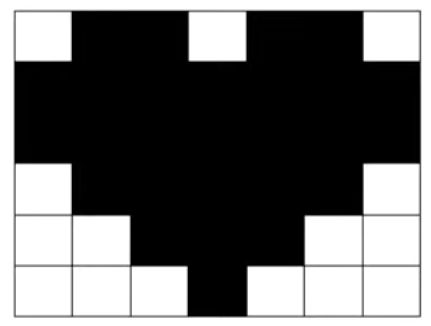
\includegraphics[width=3cm]{heart.png} \hspace{2cm}
    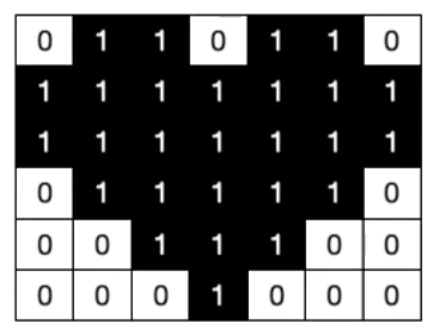
\includegraphics[width=3cm]{pixel-value-heart.png}
\end{center}

\begin{minted}[bgcolor=lightgray]{python}
# The data matrix can be represented as an numpy 2d-array like this
A = numpy.array([[0,1,1,0,1,1,0],
                 [1,1,1,1,1,1,1],
                 [1,1,1,1,1,1,1],
                 [0,1,1,1,1,1,0],
                 [0,0,1,1,1,0,0],
                 [0,0,0,1,0,0,0]])
\end{minted}

This data matrix can be decomposed into a composition of 3 matrices by using the method of Singular Value Decomposition(SVD)
$$ A_{m \times n} = U_{m \times m} \Sigma_{m \times m} V^{\top}_{n \times n} $$
Here $U$ and $V$ are orthogonal matrices and $\Sigma$ is a diagonal matrix whose diagonal entries represent the relative amount of data each rank 1 matrix that is generated by outer product of corresponding columns of $U$ and rows of $V^{\top}$ contains. \\

\begin{minted}[bgcolor=lightgray]{python}
# We can use the .svd() method from the linear algebra class of Numpy Library
U, S, V = numpy.linalg.svd(A)
\end{minted}

The above function generates the 3 matrices as follows:
\begin{equation*}
    U = \begin{bmatrix}
        -0.36 & 0 & -0.73 & -0.05 & 0.56 & 0.13 \\
        -0.54 & 0.35 & 0.27 & -0.08 & -0.16 & 0.69 \\
        -0.54 & 0.35 & 0.27 & -0.08 & 0.16 & -0.69 \\
        -0.45 & -0.35 & -0.27 & 0.52 & -0.56 & -0.13 \\
        -0.28 & -0.71 & 0.18 & -0.62 & 0 & 0 \\
        -0.08 & -0.35 & 0.46 & 0.57 & 0.56 & 0.13 \\
    \end{bmatrix}_{6\times6}
\end{equation*}

\begin{equation*}
    S = \begin{bmatrix}
        4.74 & 0 & 0 & 0 & 0 & 0 \\
        0 & 1.41 & 0 & 0 & 0 & 0 \\
        0 & 0 & 1.41 & 0 & 0 & 0 \\
        0 & 0 & 0 & 0.73 & 0 & 0 \\
        0 & 0 & 0 & 0 & 0 & 0 \\
        0 & 0 & 0 & 0 & 0 & 0 \\
    \end{bmatrix}_{6\times6}
\end{equation*}

\begin{equation*}
    V = \begin{bmatrix}
        -0.23 & -0.4 & -0.46 & -0.4 & -0.46 & -0.4 & -0.23 \\
        0.5 & 0.25 & -0.25 & -0.5 & -0.25 & 0.25 & 0.5 \\
        0.39 & -0.32 & -0.19 & 0.65 & -0.19 & -0.32 & 0.39 \\
        -0.22 & 0.42 & -0.44 & 0.42 & -0.44 & 0.42 & -0.22 \\
        0.56 & -0.43 & 0.03 & 0 & -0.03 & 0.43 & -0.56 \\
        -0.42 & -0.55 & -0.16 & 0 & 0.16 & 0.55 & 0.42 \\
        -0.12 & -0.11 & 0.69 & 0 & -0.69 & 0.11 & 0.12 \\
    \end{bmatrix}_{7\times7}
\end{equation*}

Now before moving forward let us analyse what the SVD equation represents and how it expresses the original matrix as a sum of rank 1 matrices.\\ \\

\textbf{Rank of a Matrix:} \\
Rank of a matrix is defined as the number of linearly independent column/row vectors (whichever is less in number) or in other words it is the number of zero rows in the row-reduced echelon form of the matrix. \\
For our purpose we would just need to consider the first definition of the matrix and we won't dwell into the latter definition \\
Consider the matrix given below

\begin{equation*}
    X = \begin{bmatrix}
        6 & 3 & 9 & 12 \\
        2 & 1 & 3 & 4 \\
        4 & 2 & 6 & 8 \\
        8 & 4 & 12 & 16 \\
    \end{bmatrix}_{4\times4}
\end{equation*}

Do you notice some pattern? \\
On first sight it seems that since the matrix has 4 rows and 4 columns than it's rank should be 4, but it turns out that it is not always the case. Here we observe an interesting pattern in the rows (as well as columns) of the matrix. Notice that

\begin{equation}
    R_{1} = 3 \times R_{2}
\end{equation}
\begin{equation}
    R_{3} = 2 \times R_{2}
\end{equation}
\begin{equation}
    R_{4} = 4 \times R_{2}
\end{equation}

So after this analysis we observe that actually the rank of the given matrix is just 1 and not 4. \\ \\

\textbf{Vector Outer Product:} \\
You might be familiar with the vector inner product which is just the dot product of two vectors, the result of dot/inner product of two vectors is a single scalar quantity which is the summation of products of respective elements of the vectors (note that both the vectors must have same number of elements in them for inner product to exist) \\

\begin{center}
    $\vec{x}\cdot\vec{y} = \sum_{i=1}^{n} x_{i}y_{i}$, \
    $ where \ ||\vec{x}|| = ||\vec{y}|| = n$
\end{center}

On the other hand outer product of two vectors produces an $m \times n$ matrix where $||\vec{x}|| = m$ and $||\vec{y}|| = n$. The outer product of $\vec{x}$ and $\vec{y}$ is the same as the product $\vec{x}\vec{y}^{\top}$ where $\vec{x}$ and $\vec{y}$ are both column vectors.

$$
{\displaystyle 
    \mathbf {x} \otimes \mathbf {y} =\mathbf{x}\mathbf{y^{\top}} =\mathbf {A} =
    {\begin{bmatrix} 
        x_{1}y_{1} & x_{1}y_{2} & \dots & x_{1}y_{n} \\ 
        x_{2}y_{1} & x_{2}y_{2} & \dots & x_{2}y_{n} \\ 
        \vdots & \vdots & \ddots & \vdots \\ 
        x_{m}y_{1} & x_{m}y_{2} & \dots & x_{m}y_{n}
    \end{bmatrix}_{m \times n}}
}
$$

Let us take the previous example and try to visualise what is actually happening. \\
The matrix $A$ can be written as the outer product of two vectors

$$
\mathbf{a} = {
\begin{bmatrix}
    3 \\
    1 \\
    2 \\
    4
\end{bmatrix}_{4 \times 1}
} \ and \
\mathbf{b^{\top}} = {
\begin{bmatrix}
    2 & 1 & 3 & 4
\end{bmatrix}_{1 \times 4}
}
$$

So basically outer product is nothing but the scaling of vector $b^{\top}$ by different factors given by $\begin{bmatrix}
    \vec{a}
\end{bmatrix}_{i}$ to get the $row_{i}$ of matrix A. So if we repeat the process for all the rows we get out matrix A.

$$
{\displaystyle 
    \mathbf {a} \otimes \mathbf {b} =\mathbf{a}\mathbf{b^{\top}} =\mathbf {A} =
    {\begin{bmatrix} 
        a_{1}b_{1} & a_{1}b_{2} & a_{1}b_{3} & a_{1}b_{4} \\ 
        a_{2}b_{1} & a_{2}b_{2} & a_{2}b_{3} & a_{2}b_{4} \\
        a_{3}b_{1} & a_{3}b_{2} & a_{3}b_{3} & a_{3}b_{4} \\
        a_{4}b_{1} & a_{4}b_{2} & a_{4}b_{3} & a_{4}b_{4} \\
    \end{bmatrix}} = 
    {\begin{bmatrix} 
        6 & 3 & 9 & 12 \\
        2 & 1 & 3 & 4 \\
        4 & 2 & 6 & 8 \\
        8 & 4 & 12 & 16 \\
    \end{bmatrix}}
}
$$ 

\begin{center}
    \textbf{\large Visualization}
\end{center}

\begin{center}
    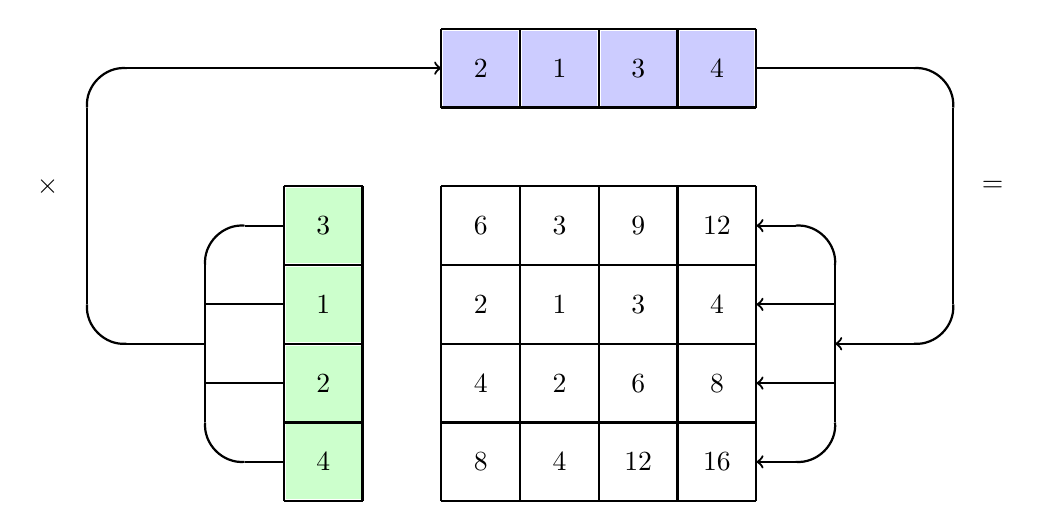
\begin{tikzpicture}
        \draw[thick] (2,0) grid(6,-1);
        \draw[thick] (0,-2) grid(1,-6);
        \draw[thick] (2,-2) grid(6,-6);
        
        \node [fill=blue!20, minimum width=0.95cm, minimum height=0.95cm] at (2.5,-0.5) {2};
        \node [fill=blue!20, minimum width=0.95cm, minimum height=0.95cm] at (3.5,-0.5) {1};
        \node [fill=blue!20, minimum width=0.95cm, minimum height=0.95cm] at (4.5,-0.5) {3};
        \node [fill=blue!20, minimum width=0.95cm, minimum height=0.95cm] at (5.5,-0.5) {4};
        
        \node [fill=green!20, minimum width=0.95cm, minimum height=0.95cm] at (0.5,-2.5) {3};
        \node [fill=green!20, minimum width=0.95cm, minimum height=0.95cm] at (0.5,-3.5) {1};
        \node [fill=green!20, minimum width=0.95cm, minimum height=0.95cm] at (0.5,-4.5) {2};
        \node [fill=green!20, minimum width=0.95cm, minimum height=0.95cm] at (0.5,-5.5) {4};
        
        \node at (2.5,-2.5) {6};
        \node at (3.5,-2.5) {3};
        \node at (4.5,-2.5) {9};
        \node at (5.5,-2.5) {12};
        
        \node at (2.5,-3.5) {2};
        \node at (3.5,-3.5) {1};
        \node at (4.5,-3.5) {3};
        \node at (5.5,-3.5) {4};
        
        \node at (2.5,-4.5) {4};
        \node at (3.5,-4.5) {2};
        \node at (4.5,-4.5) {6};
        \node at (5.5,-4.5) {8};
        
        \node at (2.5,-5.5) {8};
        \node at (3.5,-5.5) {4};
        \node at (4.5,-5.5) {12};
        \node at (5.5,-5.5) {16};

        \draw [thick] (-0.5,-2.5) -- (0,-2.5);
        \draw [thick] (-1,-3.5) -- (0,-3.5);
        \draw [thick] (-1,-4.5) -- (0,-4.5);
        \draw [thick] (-0.5,-5.5) -- (0,-5.5);

        \draw [thick] (-0.5, -2.5) edge [bend right=50] (-1, -3);
        \draw [thick] (-1, -3) -- (-1, -5);
        \draw [thick] (-0.5, -5.5) edge [bend left=50] (-1, -5);

        \draw [thick] (-1, -4) -- (-2, -4);
        \draw [thick] (-2, -4) edge [bend left=50] (-2.5, -3.5);
        \draw [thick] (-2.5, -3.5) -- (-2.5, -1);
        \draw [thick] (-2.5, -1) edge [bend left=50] (-2, -0.5);
        \draw [->, thick] (-2, -0.5) -- (2, -0.5);

        \node at (-3,-2) {$\times$};

        \draw [thick] (6, -0.5) -- (8, -0.5);
        \draw [thick] (8, -0.5) edge [bend left=50] (8.5, -1);

        \draw [<-, thick] (6,-2.5) -- (6.5,-2.5);
        \draw [<-, thick] (6,-3.5) -- (7,-3.5);
        \draw [<-, thick] (6,-4.5) -- (7,-4.5);
        \draw [<-, thick] (6,-5.5) -- (6.5,-5.5);

        \draw [thick] (6.5, -2.5) edge [bend left=50] (7, -3);
        \draw [thick] (7, -3) -- (7, -5);
        \draw [thick] (6.5, -5.5) edge [bend right=50] (7, -5);

        \draw [thick] (8.5, -1) -- (8.5, -3.5);
        \draw [thick] (8.5,-3.5) edge [bend left=50] (8, -4);
        \draw [->, thick] (8, -4) -- (7, -4);

        \node at (9,-2) {=};
    \end{tikzpicture}
\end{center}

Having the knowledge of Rank of a matrix and outer product of two vectors we can go ahead in our journey. So how does the SVD decomposition represents the original matrix as the sum of rank 1 matrices? We can answer this question now with our knowledge of rank of matrices and outer product of vectors. Note that S ($\Sigma$) is a diagonal matrix so when U is multiplied with S it is just as scaling each corresponding column vector of U with the corresponding diagonal entry, that is, if 

$$
U_{m \times m} = \begin{bmatrix}
    \vec{u}_{1} & \vec{u}_{2} & \dots &\vec{u}_{m}
\end{bmatrix}
$$ and
$$
\Sigma_{m \times m} = diag(\begin{matrix}
    \sigma_{1} & \sigma_{2} & \dots & \sigma_{m}
\end{matrix})
$$ than
$$
U\Sigma = \begin{bmatrix}
    \vec{u}_{1}\sigma_{1} & \vec{u}_{2}\sigma_{2} & \dots & \vec{u}_{m}\sigma_{m}
\end{bmatrix}
= \begin{bmatrix}
    \sigma_{1} \vec{u}_{1} & \sigma_{2} \vec{u}_{2} & \dots & \sigma_{m} \vec{u}_{m}
\end{bmatrix}
$$

Now right multiplying both sides by $V^{\top}$ we get

$$
U\Sigma V^{\top} = \begin{bmatrix} \sigma_{1} \vec{u}_{1} & \sigma_{2} \vec{u}_{2} & \dots & \sigma_{m} \vec{u}_{m} \end{bmatrix}
\begin{bmatrix}
    \vec{v}_{1}^{\top} \\
    \vec{v}_{2}^{\top} \\
    \vdots \\
    \vec{v}_{n}^{\top}
\end{bmatrix}
$$
$$
\therefore [U\Sigma V^{\top}]_{i} = \sigma_{i} (\vec{u}_{i} \otimes \vec{v}^{\top}_{i})
$$

Note that here $\vec{v}_{i}$ are row vectors and $\vec{u}_{i}$ are column vectors so here we will be doing vector outer product (also you can notice that the dimensions of the two matrices are not multiplication compatible.

\begin{center}
    \textbf{\large Visualization}
\end{center}

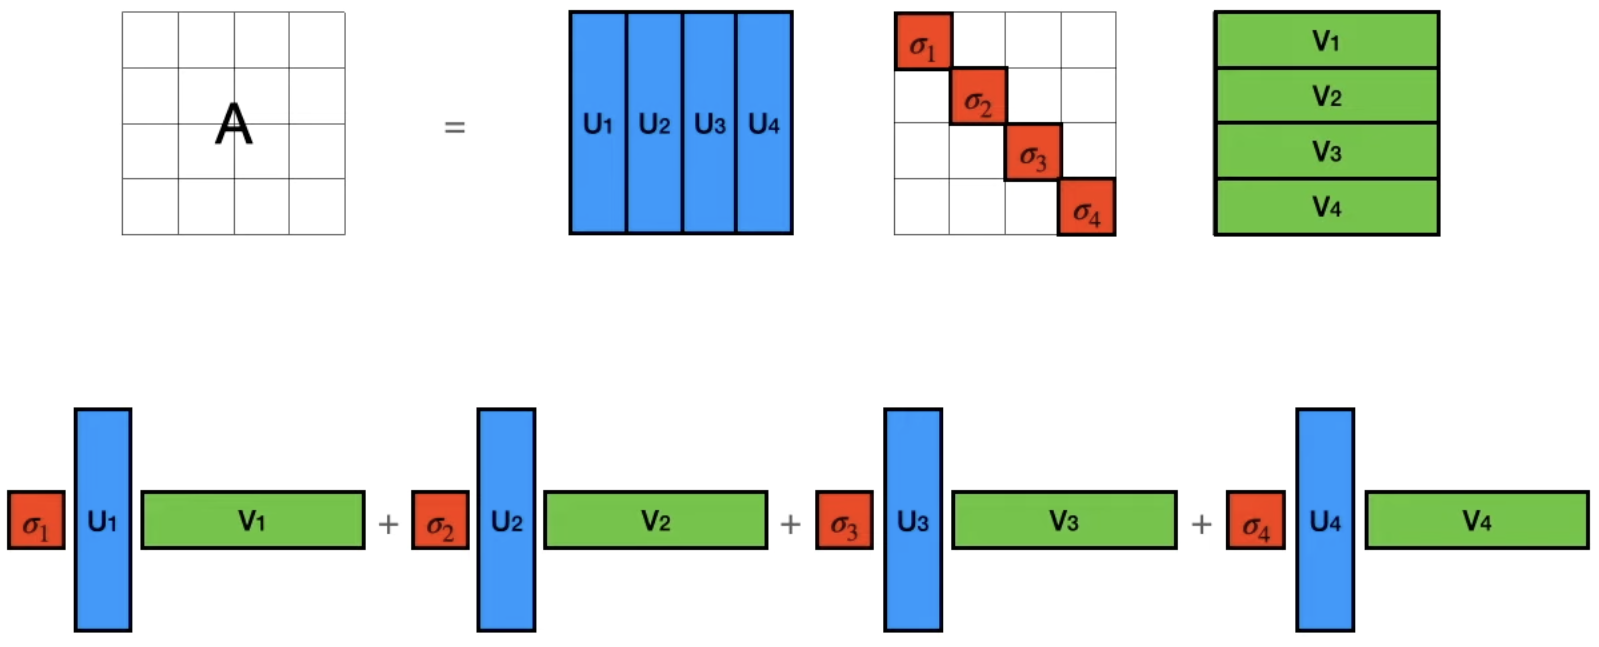
\includegraphics[width=16.5cm]{SVD_visualization.png}

Here in the figure each of the summation term is a rank 1 matrix as all the rows of a matrix in particular term is the linear combination of the vectors $\vec{v}_{i}$ according to $\vec{u}_{i}$s. So now we have decomposed our original matrix as a sum of rank 1 matrices. The amount of relative information contained in each rank 1 matrix about the original matrix is given by the associated $\sigma_{i}$, so now we want to approximate our original matrix in terms of the sum of rank 1 matrices we can drop those matrices in this expansion whose $\sigma$ coefficient is very small.
The first term in the matrix example that we are working with will be

$$
\adjustbox{valign=c}{
  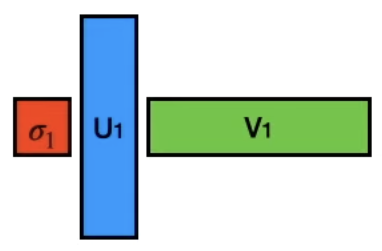
\includegraphics[width=4cm]{sig1U1V1.png}
}  = (4.74) \begin{bmatrix}
    -0.36 \\
    -0.54 \\
    -0.54 \\
    -0.45 \\
    -0.28 \\
    -0.08
\end{bmatrix}
\begin{bmatrix}
    -0.23 & 0.5 & 0.39 & -0.22 & 0.56 & -0.42 & -0.12
\end{bmatrix}
$$
$$
= (4.74) \begin{bmatrix}
    0.08 & -0.18 & -0.14 & 0.07 & -0.20 & 0.15 & 0.04 \\
    0.12 & -0.27 & -0.21 & 0.11 & -0.30 & 0.23 & 0.06 \\
    0.12 & -0.27 & -0.21 & 0.12 & -0.30 & 0.23 & 0.06 \\
    0.10 & -0.22 & -0.17 & 0.09 & -0.25 & 0.18 & 0.05 \\
    0.06 & -0.14 & -0.10 & 0.06 & -0.16 & 0.12 & 0.03 \\
    0.01 & -0.04 & -0.03 & 0.02 & -0.04 & 0.03 & 0.01
\end{bmatrix}
$$

Similarly we calculate the data matrix for each term in the summation.
After multiplying the $\sigma$ into the matrix and plotting the image from the matrix treating each entry as the value of the pixel we get the following. The value written at the top of each image indicates the respective rank 1 matrix that it represents.

\begin{minted}[bgcolor=lightgray]{python}
# All the layers in python can be generated by this code (taking outer product)
# array to store all the layers
array_of_layers = []
for layer in range(len(U[0])): # number of layers = number of columns of U
    img_layer = [] # each layer would be a 2D matrix
    colU = []
    rowV = V[layer]
    for row in range(len(U)):
        colU.append(U[row][layer])
    sigma = S[layer]
    for row in range(len(colU)):
        r = []
        for i in range(len(rowV)):
            r.append(colU[row] * rowV[i] * sigma)
        img_layer.append(r)
    array_of_layers.append(img_layer)
\end{minted}

\begin{center}
    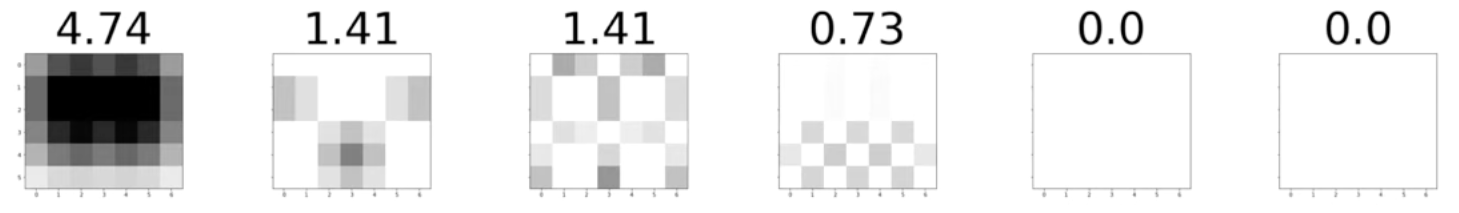
\includegraphics[width=16.5cm]{components.png}
\end{center}

The above images can be represented as different layers of the original image so as we go on putting one layer on top of the other our original image starts to form. As we keep adding more and more terms we get colser and closer to our original image. On adding these images on top of one another we get the following:

\begin{minted}[bgcolor=lightgray]{python}
# The masked images can be generated by the following code
array_of_masked_images = []
for layer in array_of_layers:
    if len(array_of_masked_images) == 0:
        array_of_masked_images.append(layer)
        pass
    else:
        prev_img = array_of_masked_images[-1]
        curr_layer = layer
        # generates a zero array of the dimensions of the image
        new_image = [[0 for _ in range(len(prev_img[0]))] for _ in range(len(prev_img))]
        for i in range(len(curr_layer)):
            for j in range(len(curr_layer[0])):
                new_image[i][j] += prev_img[i][j] + curr_layer[i][j]
        array_of_masked_images.append(new_image)
\end{minted}

\begin{center}
    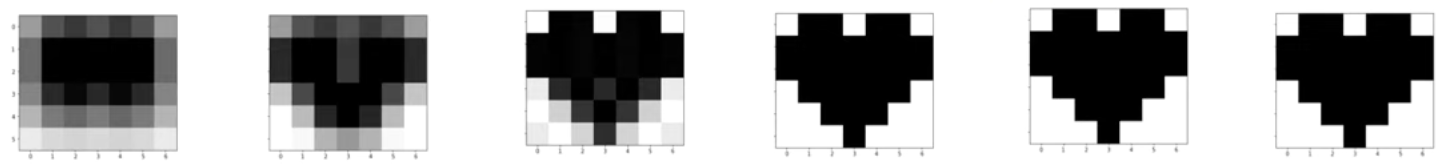
\includegraphics[width=16.5cm]{masked_images.png}
\end{center}

This shows that even if we just store the first three layers we get a pretty good approximation of our original image without loosing much information (Note that here the number of layers is quiet low so it does not make sense to store just a few parts as the image is already very low resolution but in case of high resolution images this methods makes a significant difference). If we just store the first three layers than the total number of values we will need to store is the first three columns of $U$ and first three columns of $V$ (or first three rows of $V^{\top}$, that is $\implies (3 \times 6) + (3 \times 7) = 18 + 21 = 39$ values (Since we can easily generate the image by taking the outer products of the respective vectors and adding each 1 rank matrix)(Also note that we need not explicitely store the $\sigma$ values as it can be first multiplied into the respective columns of $U$ and then those columns can be directly stored). Which is less than the $7 \times 6 = 42$ values that we would need to store for the original image(Although it is not much in this case but for higher resolution images this is a significant number, for example for a image containing 4000 x 4000 resolution if we even store just the first 100 columns(with retaining more than 95\% of quality) of respective $U$ and $V$ matrices we would just need to store 8,00,000 values as compared to 1,60,00,000 values we would otherwise need to store for the original image).

\end{document}
